\chapter{DATASET, DATABASE AND DESIGN OF THE NDVI APPLICATION}
\label{chap:argo}

\section{NDVI dataset and its significance}

\subsection{About MODIS}

\newcommand{\MYhref}[3][blue]{\href{#2}{\color{#1}{#3}}}%

\centerline{\MYhref{https://modis.gsfc.nasa.gov/}{NASA's MODIS website}}

\gls{modis} is a key instrument on board the Terra (initially known as EOS AM-1) and Aqua (initially known as EOS PM-1) satellites. Land's circle around the Earth is coordinated with the goal that it goes from north to south over the equator early in the day, while Aqua disregards south to north the equator toward the evening. Land \gls{modis} and Aqua \gls{modis} are seeing the whole Earth's surface each 1 to 2 days, gaining information in 36 ghastly groups, or gatherings of wavelengths (see \gls{modis} Technical Specifications). These information will enhance our comprehension of worldwide elements and procedures happening on the land, in the seas, and in the lower climate. \gls{modis} is assuming a fundamental job in the improvement of approved, worldwide, intuitive Earth framework models ready to foresee worldwide change precisely enough to help arrangement creators in settling on quality choices concerning the security of our condition. \\

\subsection{Overview of NDVI Dataset}

\gls{modis} vegetation indices, delivered on 16-day interims and at various spatial goals, give steady spatial and worldly correlations of vegetation covering greenness, a composite property of leaf territory, chlorophyll and shade structure. Two vegetation lists are gotten from environmentally redressed reflectance in the red, close infrared, and blue wavebands; the standardized contrast vegetation list \gls{ndvi}, which gives coherence \gls{noaa}'s AVHRR \gls{ndvi} time arrangement record for verifiable and atmosphere applications, and the upgraded vegetation list (EVI), which limits covering soil varieties and enhances affectability over thick vegetation conditions. The two items all the more successfully describe the worldwide scope of vegetation states and procedures. 

The vegetation records are recovered from day by day, air redressed, bidirectional surface reflectance. The VI's utilization a \gls{modis}-particular compositing strategy dependent on item quality confirmation measurements to evacuate low quality pixels. From the staying great quality VI esteems, an obliged see edge approach at that point chooses a pixel to speak to the compositing time frame (from the two most elevated \gls{ndvi} esteems it chooses the pixel that is nearest to-nadir). Since the \gls{modis} sensors on board Terra and Aqua satellites are indistinguishable, the VI calculation creates every 16-day composite eight days separated (staged items) to allow a higher worldly goals item by joining the two information records. The \gls{modis} VI item suite is currently utilized effectively in all environment, atmosphere, and regular assets administration contemplates and operational research as exhibited by the consistently expanding group of associate distributions. \\

\centerline{\textbf{How do you calculate NDVI?}}

\textbf{\[ NDVI = \frac{NIR - RED}{NIR + RED} \ \ \ 
\ \ \]}

\centerline{NIR: \gls{nir}}
\centerline{RED: \gls{red}}

Solid vegetation (chlorophyll) reflects more close \gls{nir} and green light contrasted with different wavelengths. In any case, it retains more red and blue light. 

This is the reason our eyes consider vegetation to be the shading green.

Let's look at the example shown in the fig 3.1.

    \begin{figure}[H]
            \centering
            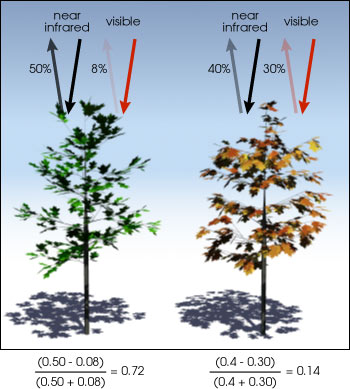
\includegraphics[width=0.5\linewidth]{figures/ch3/ndvi-example.png}
            \caption{\label{fig:level_list_screen} NDVI Example - Courtsey: NASA}
    \end{figure}

Data is normally stored in a \gls{gdac} \gls{ftp} server, at a US-based server at \url{https://gimms.gsfc.nasa.gov/MODIS/}.

The information is thought to be adequately quality controlled and in a steady arrangement. Stage and profile name is the main distinguishing proof. This information structure does not permit regular determination or spatial choice: a key element to any atmosphere informational index. The FTP server is intended to go about as a chronicle. Researchers are urged to download the information locally for their utilization's, a procedure that depends on noteworthy space learning of the FTP website. Barely any individuals will experience the inconvenience of understanding the FTP structure, less still will set aside opportunity to make the procedure less demanding for other people.

\subsection{Significance}

The term \gls{ndvi} in the farming business has positively increased more mindfulness of late because of the developing ubiquity of little unmanned elevated vehicles. 

\gls{ndvi} is positively not another child on the square and with regards to social affair and preparing this data, rural experts have known and been utilizing this information for quite a long time. Anyway already assembling this information may have been tedious, awkward, not exceptionally precise and costly. 

As innovation enhances and the methods in which we would now be able to catch this information, agriculturists are beginning to take this basic and successful information all the more genuinely by hoping to join this technique into their product administration methodology. 

Information is enter in exactness farming, knowing your product's well being is a certain something yet really pre-empting the state of harvest's well being, endorsing compost application, distinguish any potential sickness and precisely assessing yield puts the control in your grasp consequently making you all around educated to settle on the correct business choices as and when required.

\gls{ndvi} is valuable for evaluating the well being and thickness of vegetation. \gls{ndvi} esteems close to 0 show extremely inadequate vegetation. Thick vegetation is demonstrated by \gls{ndvi} esteems moving toward 1. By utilizing a period arrangement of \gls{ndvi} perceptions, one can look at the elements of the developing season and screen wonders, for example, dry spell. A full supplement of information has been finished from the earliest starting point of Terra satellite activity to the present and is accessible for download in peruse and 250m goals.


\section{Wireframes Designs}



\section{Database Architecture}



